\documentclass[10pt]{beamer}
\usetheme{CambridgeUS}
\usecolortheme{beaver}
\usepackage{graphicx}
\usepackage{color}
\usepackage{mathptmx}
\usepackage{geometry}
\usepackage{multicol}
\usepackage{hyperref}
\usepackage{threeparttable}
\usepackage{array} % for adding extra space between table columns
\usepackage{booktabs} % for adding extra space between table columns
\usepackage{multirow}

\colorlet{shadecolor}{blue!15}
\newtheorem{prop}{Proposition}
\newenvironment{propc}[1]
{\begin{shaded}\begin{prop}}
		{\end{prop}\end{shaded}}

\title[Monetary Policy Spillover through Trade Channel]{Global Monetary Policy Spillover through Trade Channel}
\author[Lu\&Yao (2023)]{\large Lingfei LU, Jingbo YAO \\ \vspace{0.5cm} Department of Economics, HKUST \\ \vspace{0.5cm} HKUST-Jinan Macro Student Symposium 2023}
\date{This Version: July 2023}
\logo{
\includegraphics[scale=0.15]{UST4C_L3.eps}}

\begin{document}
	
    \begin{frame}[plain]
	\maketitle {}
    \end{frame}

%----------------------------------------

\section{Introduction}

\begin{frame}{Motivation}



\begin{itemize}
\item In a globalized era, how international \textcolor{blue}{monetary policies} transmit globally is a crucial question.
\item However, the channels are underexplored: the bank channel is well-studied, while the \textcolor{blue}{real channels} draw less attention. 
\item Now, a growing literature shows that most of the total impact is due to the network effect of \textcolor{blue}{global production linkages}.
\item \textbf{Our question}: How the \textcolor{blue}{behavior of exporters} response to global monetary shocks? Also, What's the implication for \textcolor{blue}{monetary policy spillover}?
\item We will consider these questions using \textcolor{blue}{China}, the biggest exporter in the world, as an example. 
\end{itemize}

\end{frame}



\begin{frame}{This paper}
\begin{itemize}
\item \textbf{Data}: China's customs data;  China's industry firm data; high-frequency global monetary shock data 
\item \textbf{Main results}: \textcolor{blue}{tightening} US monetary shock significantly \textcolor{blue}{increases} China's export prices. For European shock: \textcolor{blue}{decreases}. UK and Japan's effects: insignificant. 
\item \textbf{Channels}: 
\begin{itemize}
    \item Supply side dominates: US shock (+) \textcolor{blue}{marginal cost (interest expenditure)} (+) China's export prices(+); Heterogeneity across firms (YES)
    \item Demand side dominates: EU shock (+) import demand (-) China's export prices(-); Heterogeneity across firms (No)
\end{itemize} 
\item \textbf{Model}: Two-country model to justify the pricing behavior of China's export firms and illustrate that this additional channel \textcolor{blue}{exacerbates the recession} of China's export countries following a US contractionary shock.
\item \textbf{Contribution}: The first paper to empirically investigate the relationship between global monetary shock and export prices and its implication for global monetary shock transmission. 
\end{itemize}

\end{frame}

\begin{frame}{Literature}

\begin{itemize}
\item \textbf{Monetary transmission through bank channel}: 
    \begin{itemize}
        \item Cetorelli and Goldberg (2012, JF), Bruno and Shin (2015, RES).
        \item We study \textcolor{blue}{trade channel}
    \end{itemize} 
\item \textbf{Monetary transmission through real channel}: 
    \begin{itemize}
        \item Bräuning and Sheremirov (2019); Wei and Xie (2020, JIE); Di Giovanni and Hale (2022, JF); Chang, et al (2021, JFE)
        \item We focus on \textcolor{blue}{export price}
    \end{itemize}
\item \textbf{Real shock transmission through IO linkage}: 
    \begin{itemize}
        \item Eaton et al. (2016, AER); Auer, Levchenko, and Sauré (2019, RESta)
        \item We investigate \textcolor{blue}{monetary shocks}
    \end{itemize}

\item \textbf{Exchange rate pass-through}:
	\begin{itemize}
		\item Gopinath and Itskhoki (2010, QJE); Amiti,Itskhoki, and Konings (2014, AER)
            \item We consider the responses of export prices to \textcolor{blue}{monetary shocks}
	\end{itemize}
\item \textbf{China Shock}:
	\begin{itemize}
		\item Asquith, et al. (2019, JIE); Bombardini, Li, and Francesco Trebbi (2023, AER)
            \item We test China export-related \textcolor{blue}{cost shock}
	\end{itemize}
\end{itemize}
    

 
\end{frame}


\section{Empirical}

\begin{frame}{Data: Monetary Policy Shock}
    \begin{itemize}
        \item First, we use a U.S. monetary policy shock series as in \cite{brw2021}.
        \begin{itemize}
            \item This series is derived from a two-step, partial-least squares estimation using daily interest rate data across a wide spectrum of maturities.
            \item It only contains unpredictable Fed policy surprises and no significant central bank information effect.
        \end{itemize}
        \begin{figure}[htbp]
		\centering
		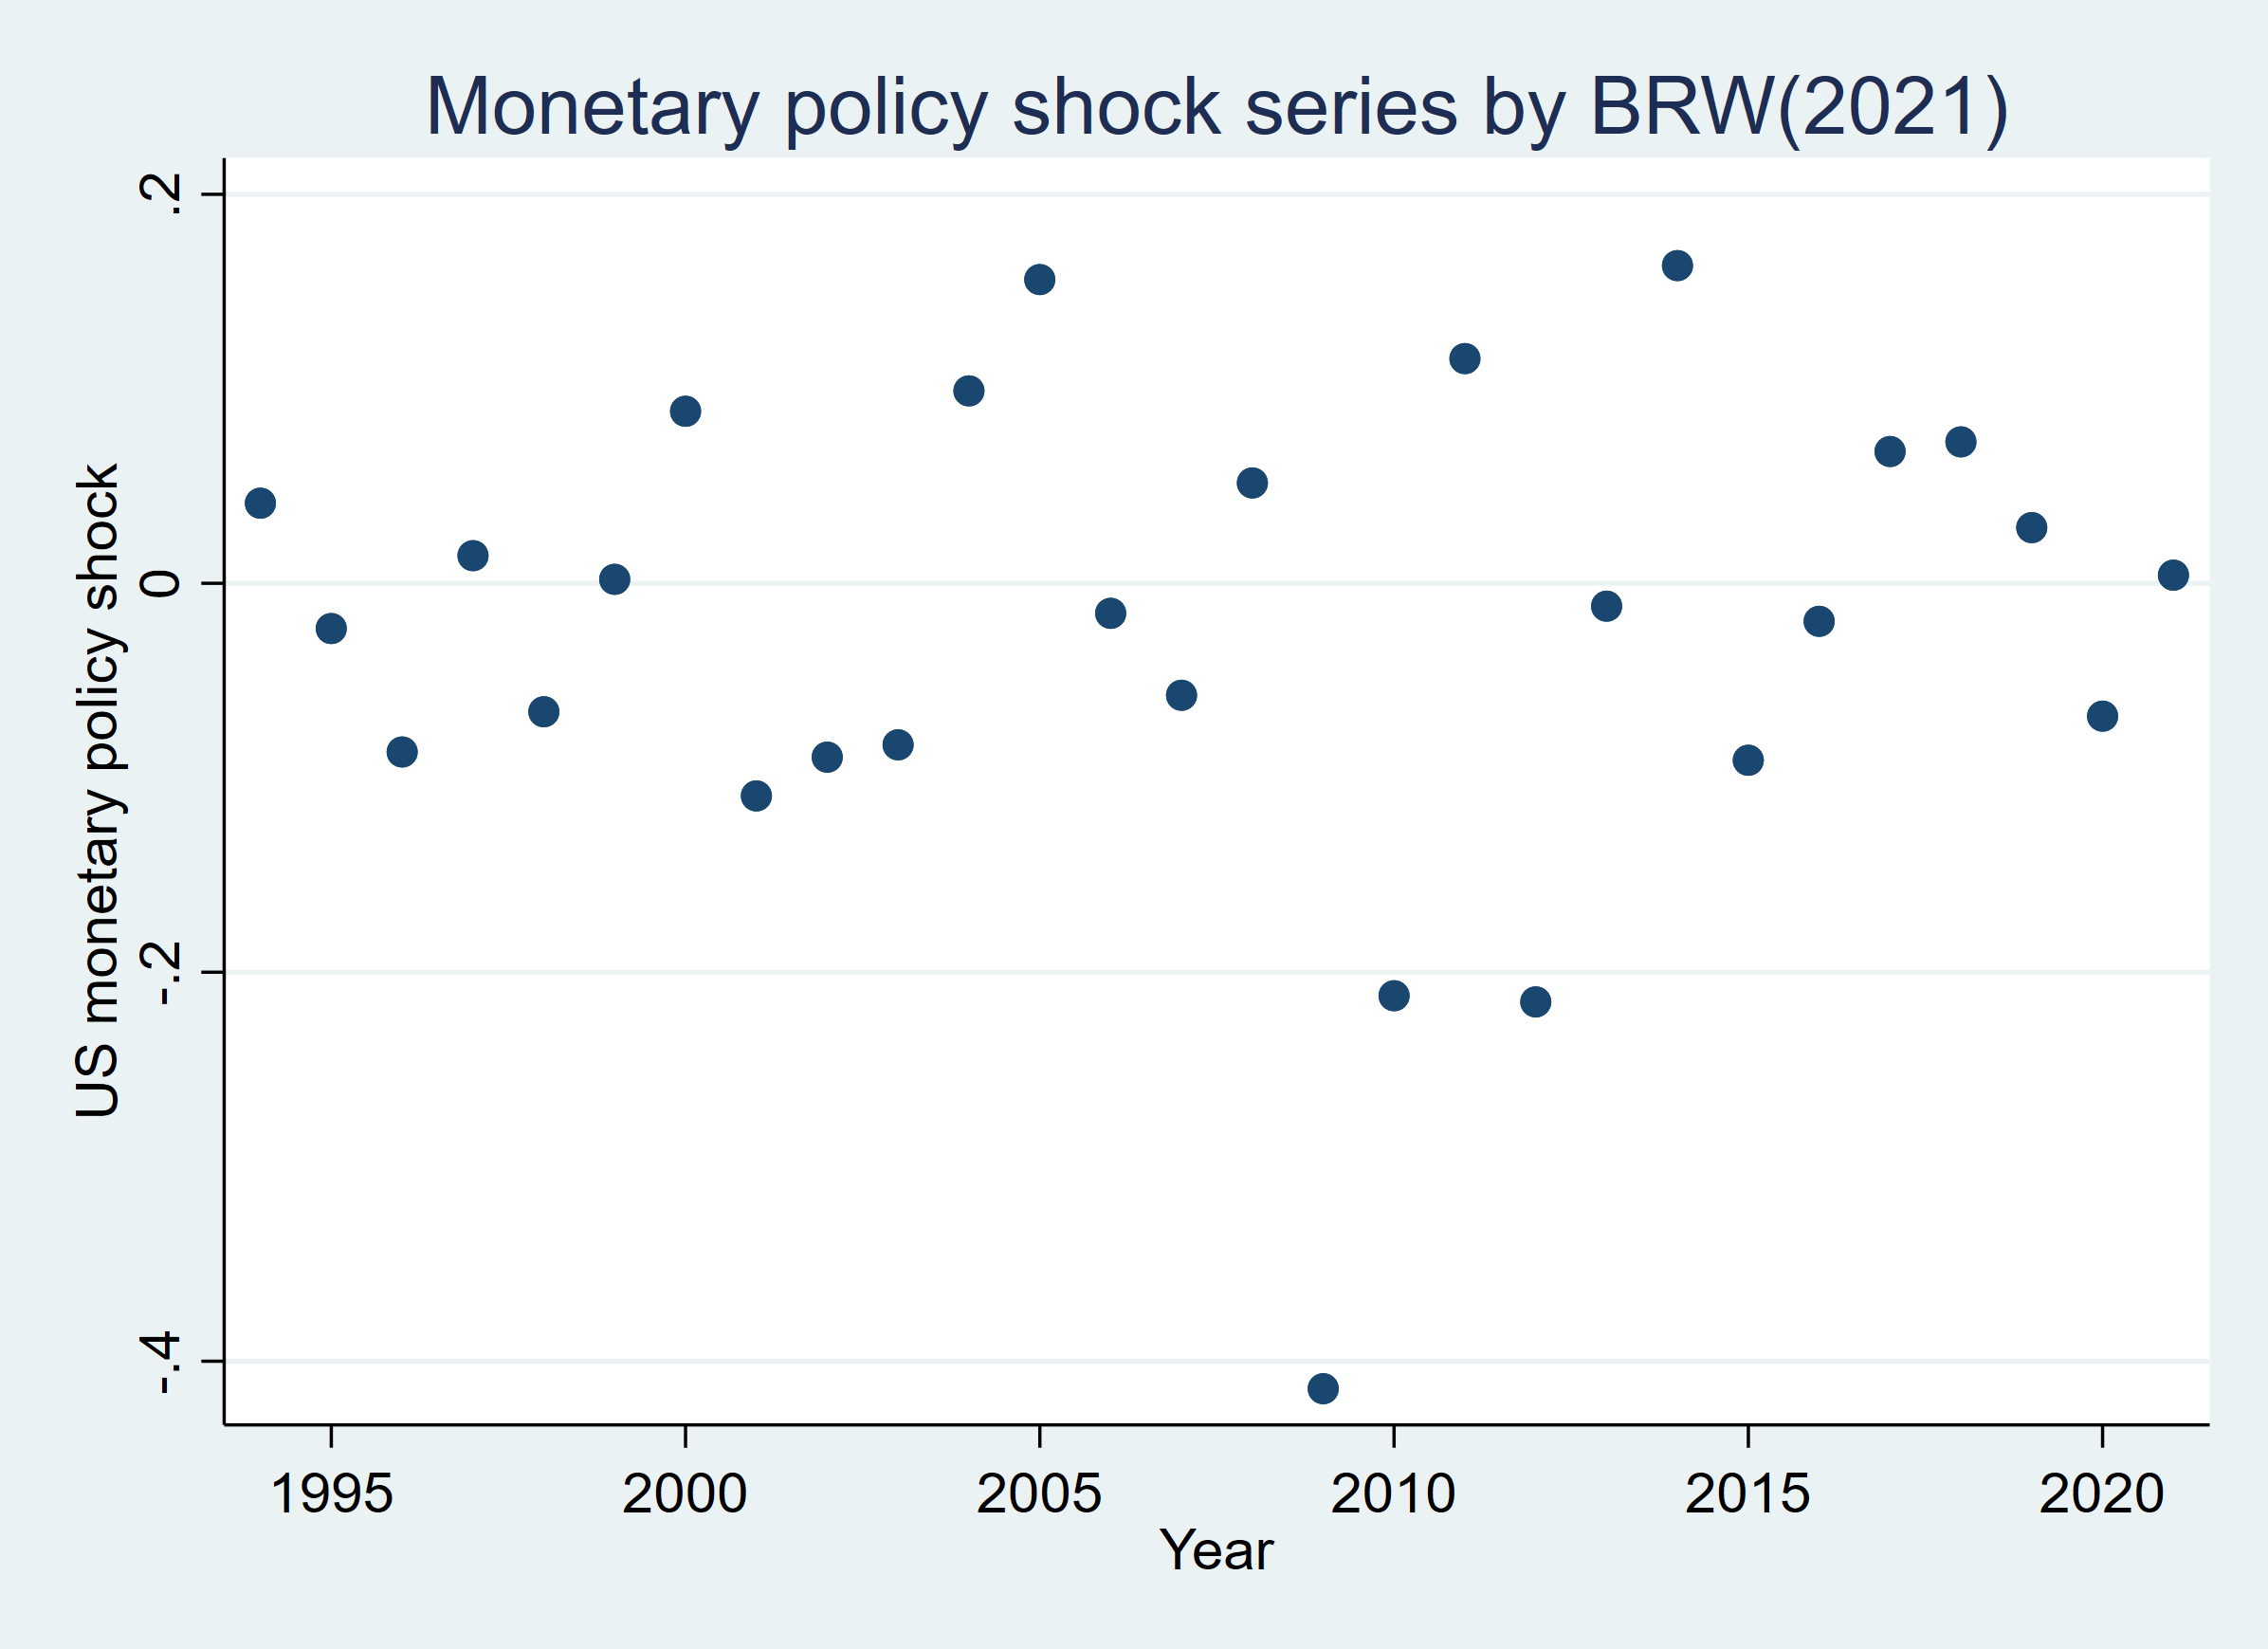
\includegraphics[width=0.65\columnwidth]{latex/slides/pic_Jun2023/BRW.png}
		\label{sum.brw}
	\end{figure}
    \end{itemize}
\end{frame}

\begin{frame}{Data: Customs Transaction Records}
	\begin{itemize}
		\item Second, we use trade transaction records from the General Administration of Customs of China (GACC).
		\begin{itemize}
			\item This dataset provides universal information on Chinese trade transactions, including import and export values, quantities, units, product names and codes, source and destination countries, and types of enterprises.
                \item The firm-level transaction records range from 2000-2011, while product-level aggregates are available until 2019.
                \item The categories of products are coded by the Harmonized Coding and Description System (HS) from the World Customs Organization (WCO).
                \item We drop unwanted observations, including products with missing information of unit or quantity, special product categories such as arms and antiques, and transactions existing for only one year.
		\end{itemize}		
	\end{itemize}
\end{frame}

\begin{frame}{Data: Firm-level Information}
	\begin{itemize}
		\item Third, we use annual surveys of Chinese manufacturing firms conducted by the National Bureau of Statistics of China (NBSC).
		\begin{itemize}
			\item This dataset covers all state-owned enterprises and above-scale firms with annual sales of more than 5 million RMB from 1999 to 2007.
			\item The data provide details about firms’ identification code, ownership, industry type, and 80 other balance sheet variables, including the number of employees, total wage payments, fixed assets, sales income, total operation inputs, etc.
		\end{itemize}
		\item To merge the firm data with customs records, we match the identification codes based on firms' contact information as in \cite{fan-li-yeaple2015}.
            \begin{itemize}
                \item The matched sample ranges from 2000 to 2007, with more than 1 million firm-product-country-year observations.
            \end{itemize}
	\end{itemize}
\end{frame}

\begin{frame}{Summary Statistics}
    \begin{table}[htbp]
        \centering
	\caption{Summary statistics for customs and firm data}
	\label{summ.sample}
        \resizebox{0.95\columnwidth}{!}
        {
	\begin{tabular}{lcccccc}
		\toprule
            & \multicolumn{1}{l}{\#observations} & \multicolumn{1}{l}{Mean} & \multicolumn{1}{l}{Median} & \multicolumn{1}{l}{Std. dev} & \multicolumn{1}{l}{P10} & \multicolumn{1}{l}{P90} \\
            \midrule
		\textbf{Panel A: Customs records} &       &       &       &       &       &  \\
		Annual Export Price Change & 11,400,795 & 0.0259 & 0.0060 & 0.6653 & -0.5001 & 0.5709 \\
		Annual Import Price Change  & 8,580,234 & 0.0236 & -0.0021 & 1.0171 & -0.8523 & 0.9388 \\
		\midrule
		\textbf{Panel B: Firm information} &       &       &       &       &       &  \\
		Sales Income (×1000 RMB) & 1,745,511 & 78826.33 & 17630 & 714350.5 & 5318  & 111319 \\
		Employment (persons)& 1,745,511 & 262.95 & 108   & 964.64 & 30    & 500 \\
		Fixed Asset (×1000 RMB) & 1,745,511 & 27437.2 & 4043  & 312024.8 & 573   & 36968 \\
		Operation Input (×1000 RMB) & 1,745,511 & 61682.99 & 13971 & 562923.1 & 4035  & 168810 \\
		Current wage payable (×1000 RMB) & 1,745,511 & 3730.16 & 1121  & 28699.16 & 266   & 6300 \\
		\midrule
		\textbf{Panel C: Matched sample} &       &       &       &       &       &  \\
		Annual Export Price Change & 1,724,591 & 0.0239 & 0.0062 & 0.6802 & -0.4828 & 0.5495 \\
		Annual Import Price Change  & 1,478,176 & -0.0902 & -0.0019 & 1.3747 & -1.2688 & 1.0616 \\
		\bottomrule
	\end{tabular}
        }
    \end{table}
\end{frame}

\begin{frame}{Baseline Empirical Strategy}
    \begin{itemize}
        \item We first estimate the unconditional impact of U.S. monetary policy shocks on Chinese exporters' annual price change (\cite{lmx2015}).
        \begin{equation}
	   \Delta \ln P_{i j c t}=\beta^P_1 M P_{t} + \beta^P_2 M P_{t-1}+ \mathbf{Z}_{jt} \boldsymbol{\gamma}^{\prime}+\mathbf{X}_{ct} \boldsymbol{\delta}^{\prime} +\xi_{i j c} + \varepsilon_{ijct}
	\label{eq.baseline}
        \end{equation}
        \item We also test whether firms significantly adjust their export quantities in the face of monetary policy shocks.
        \begin{equation}
	   \Delta \ln Q_{i j c t}=\beta^Q_1 M P_{t} + \beta^Q_2 M P_{t-1}+ \mathbf{Z}_{jt} \boldsymbol{\gamma}^{\prime}+\mathbf{X}_{ct} \boldsymbol{\delta}^{\prime} +\xi_{i j c} + \varepsilon_{ijct}
	\label{eq.quantity}
        \end{equation}
        \item The baseline US monetary policy shocks $MP^{US}_t$ are from \cite{brw2021}. We also include monetary shocks from three other major central banks, the European Central Bank, the Bank of England, and the Bank of Japan.
    \end{itemize}
\end{frame}

\begin{frame}{Baseline Empirical Strategy}
    \begin{itemize} 
        \item The export price $P_{i j c t}$ are computed as the unit value in Chinese RMB:
    		$$
    		P_{ijct}=\frac{V_{ijct}\cdot NER^US_{t}}{Q_{ijct}}
    		$$
            where value (in US dollar) $V_{ijct}$ and quantities $Q_{ijct}$ are known for each HS6 product $i$, by firm $j$, from country $c$, in year $t$.
        \item If an unexpected foreign (e.g., US) monetary policy tightening, $MP_t > 0$, raises the average export price of Chinese firms, we would expect that $\beta_1 > 0$.
        \item The coefficients $\beta_2$ of lagged terms $MP_{t-1}$ is used to isolate the impact of the previous year's monetary policy shock on the current year.
    \end{itemize}
\end{frame}

\begin{frame}{US shock vs EU shock}
    \begin{itemize}
        \item A positive \textbf{US Fed} monetary policy shock will \textbf{increase} the average export price of Chinese firms, while a positive \textbf{ECB} monetary policy shock will \textbf{decrease} the average export price.
        \begin{columns}
    	\column{0.5\columnwidth}
    	\begin{figure}[htbp]
    	   \centering
    		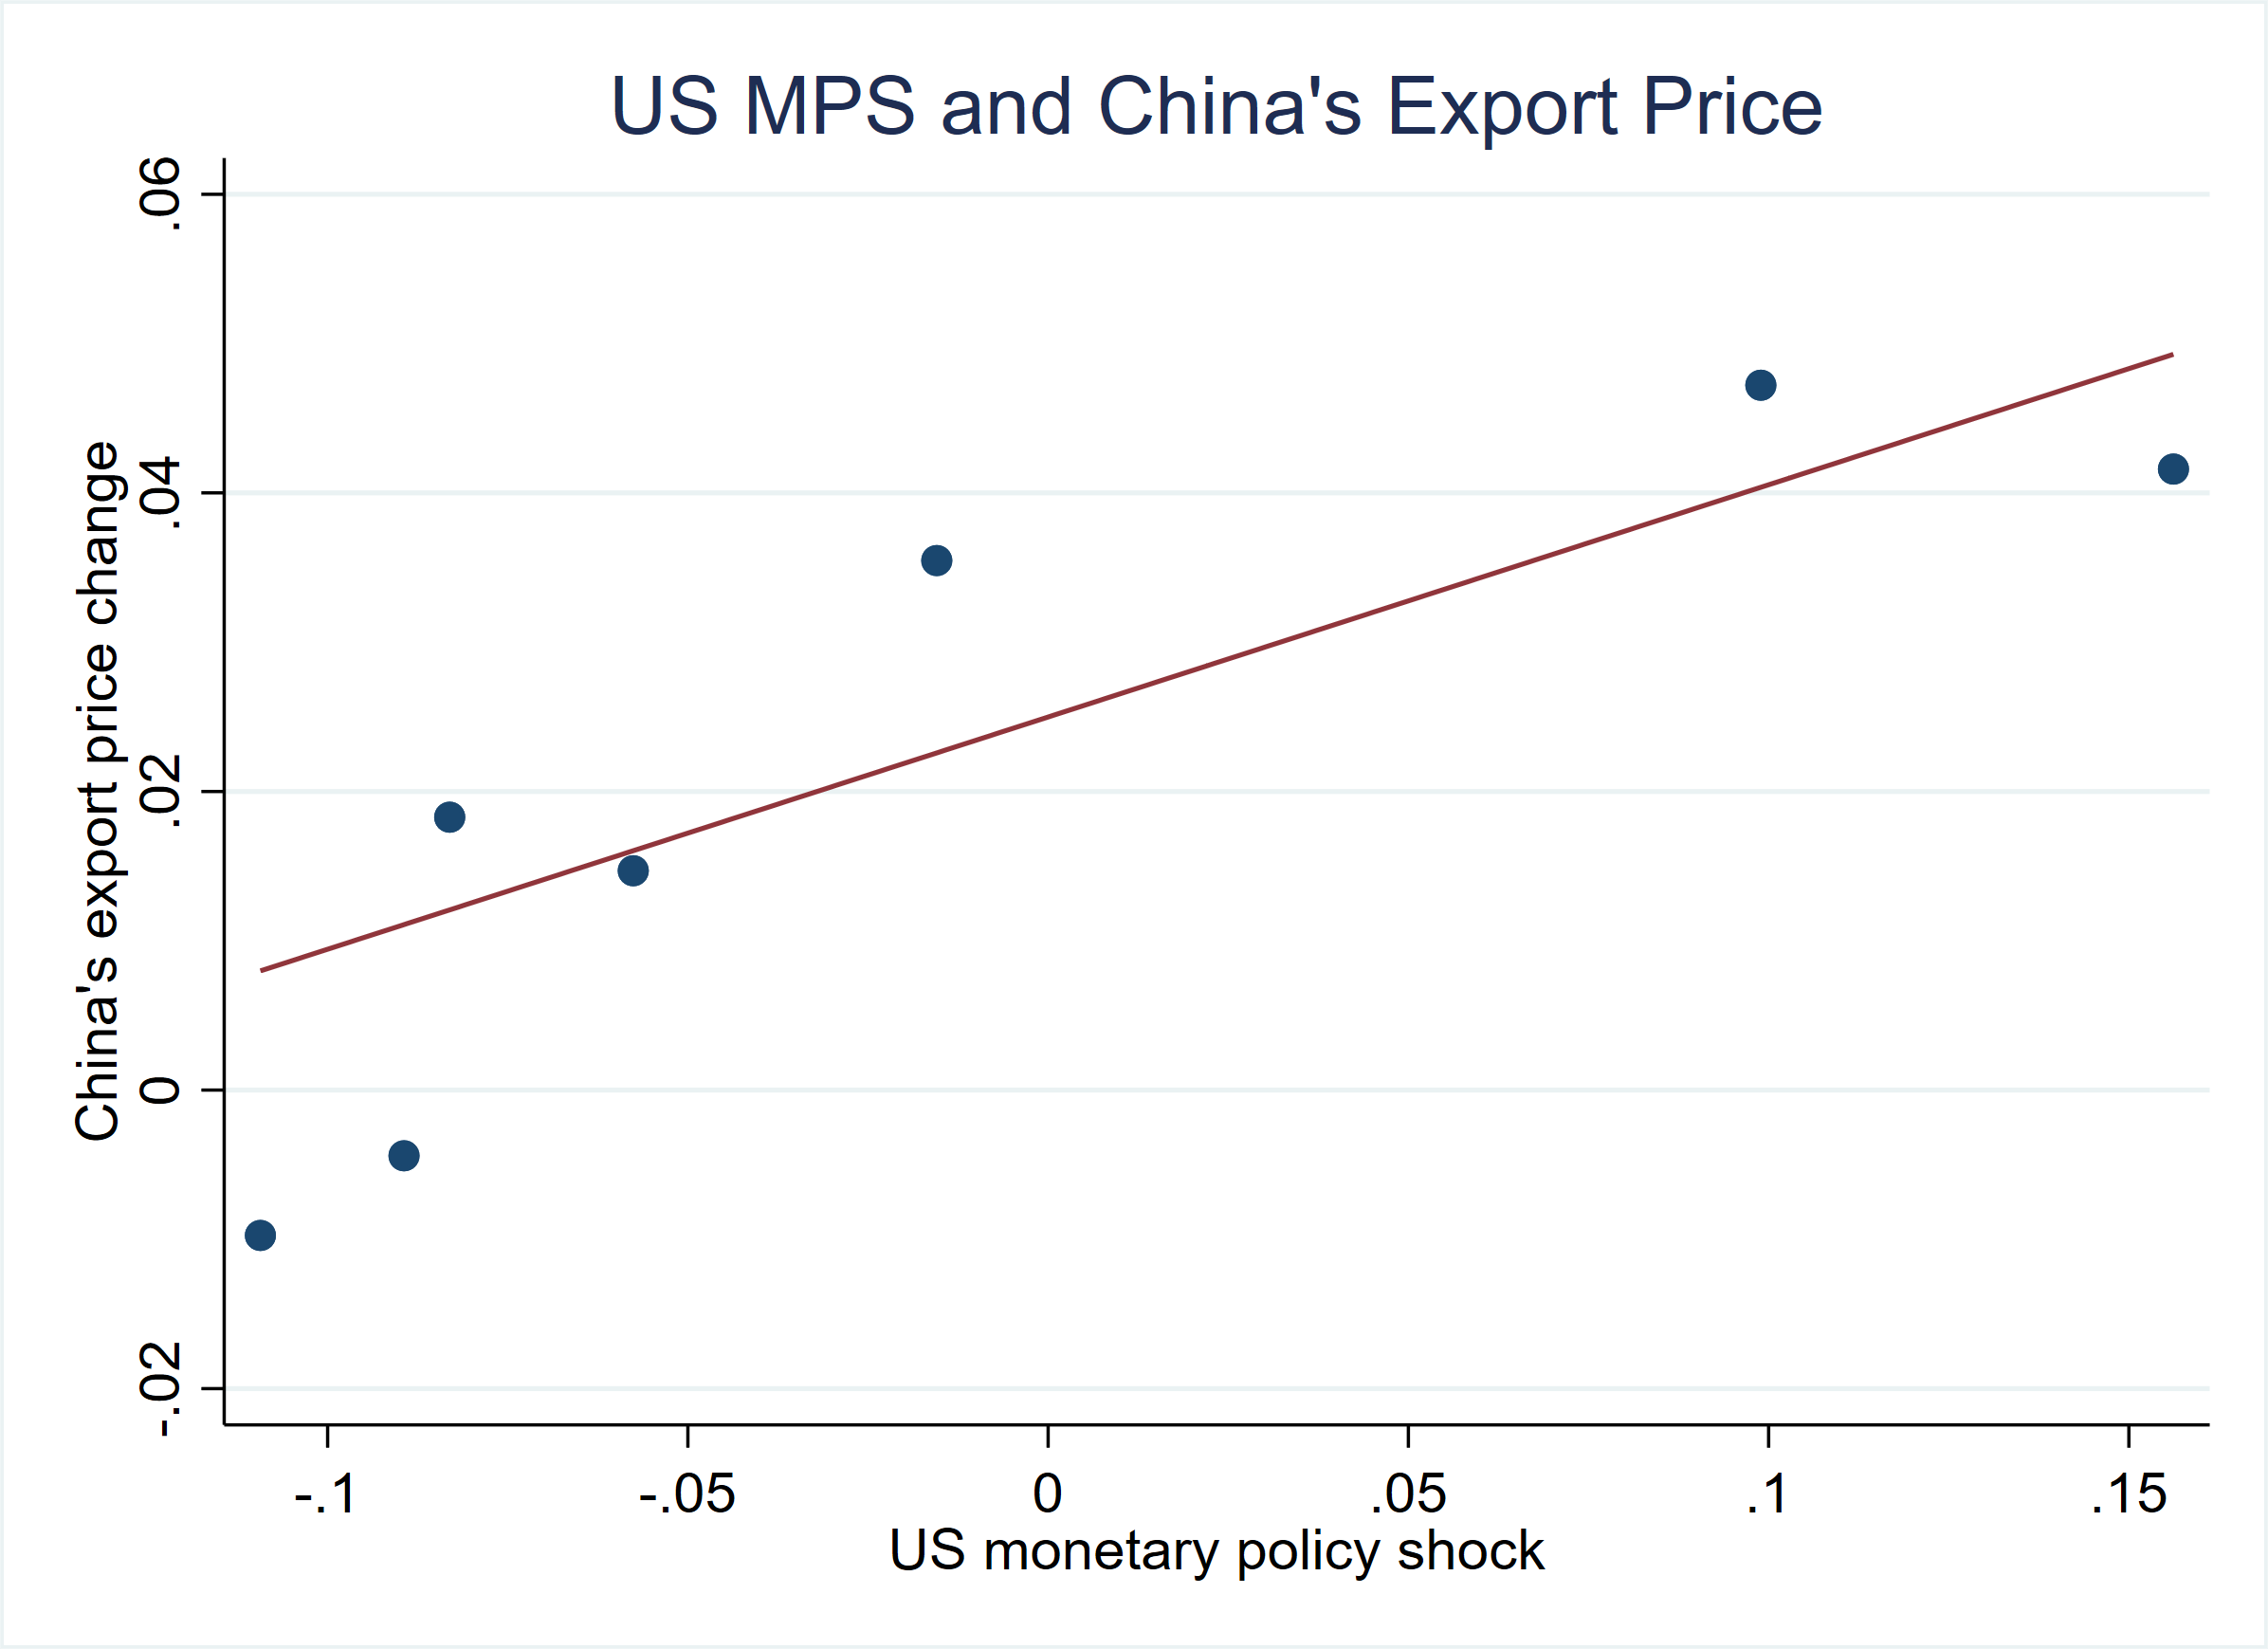
\includegraphics[width=\columnwidth]{latex/slides/pic_Jun2023/US_shock.png}
    		\label{fig.US_shock}
    	\end{figure}
    	\column{0.5\columnwidth}
    	\begin{figure}[htbp]
    		\centering
    		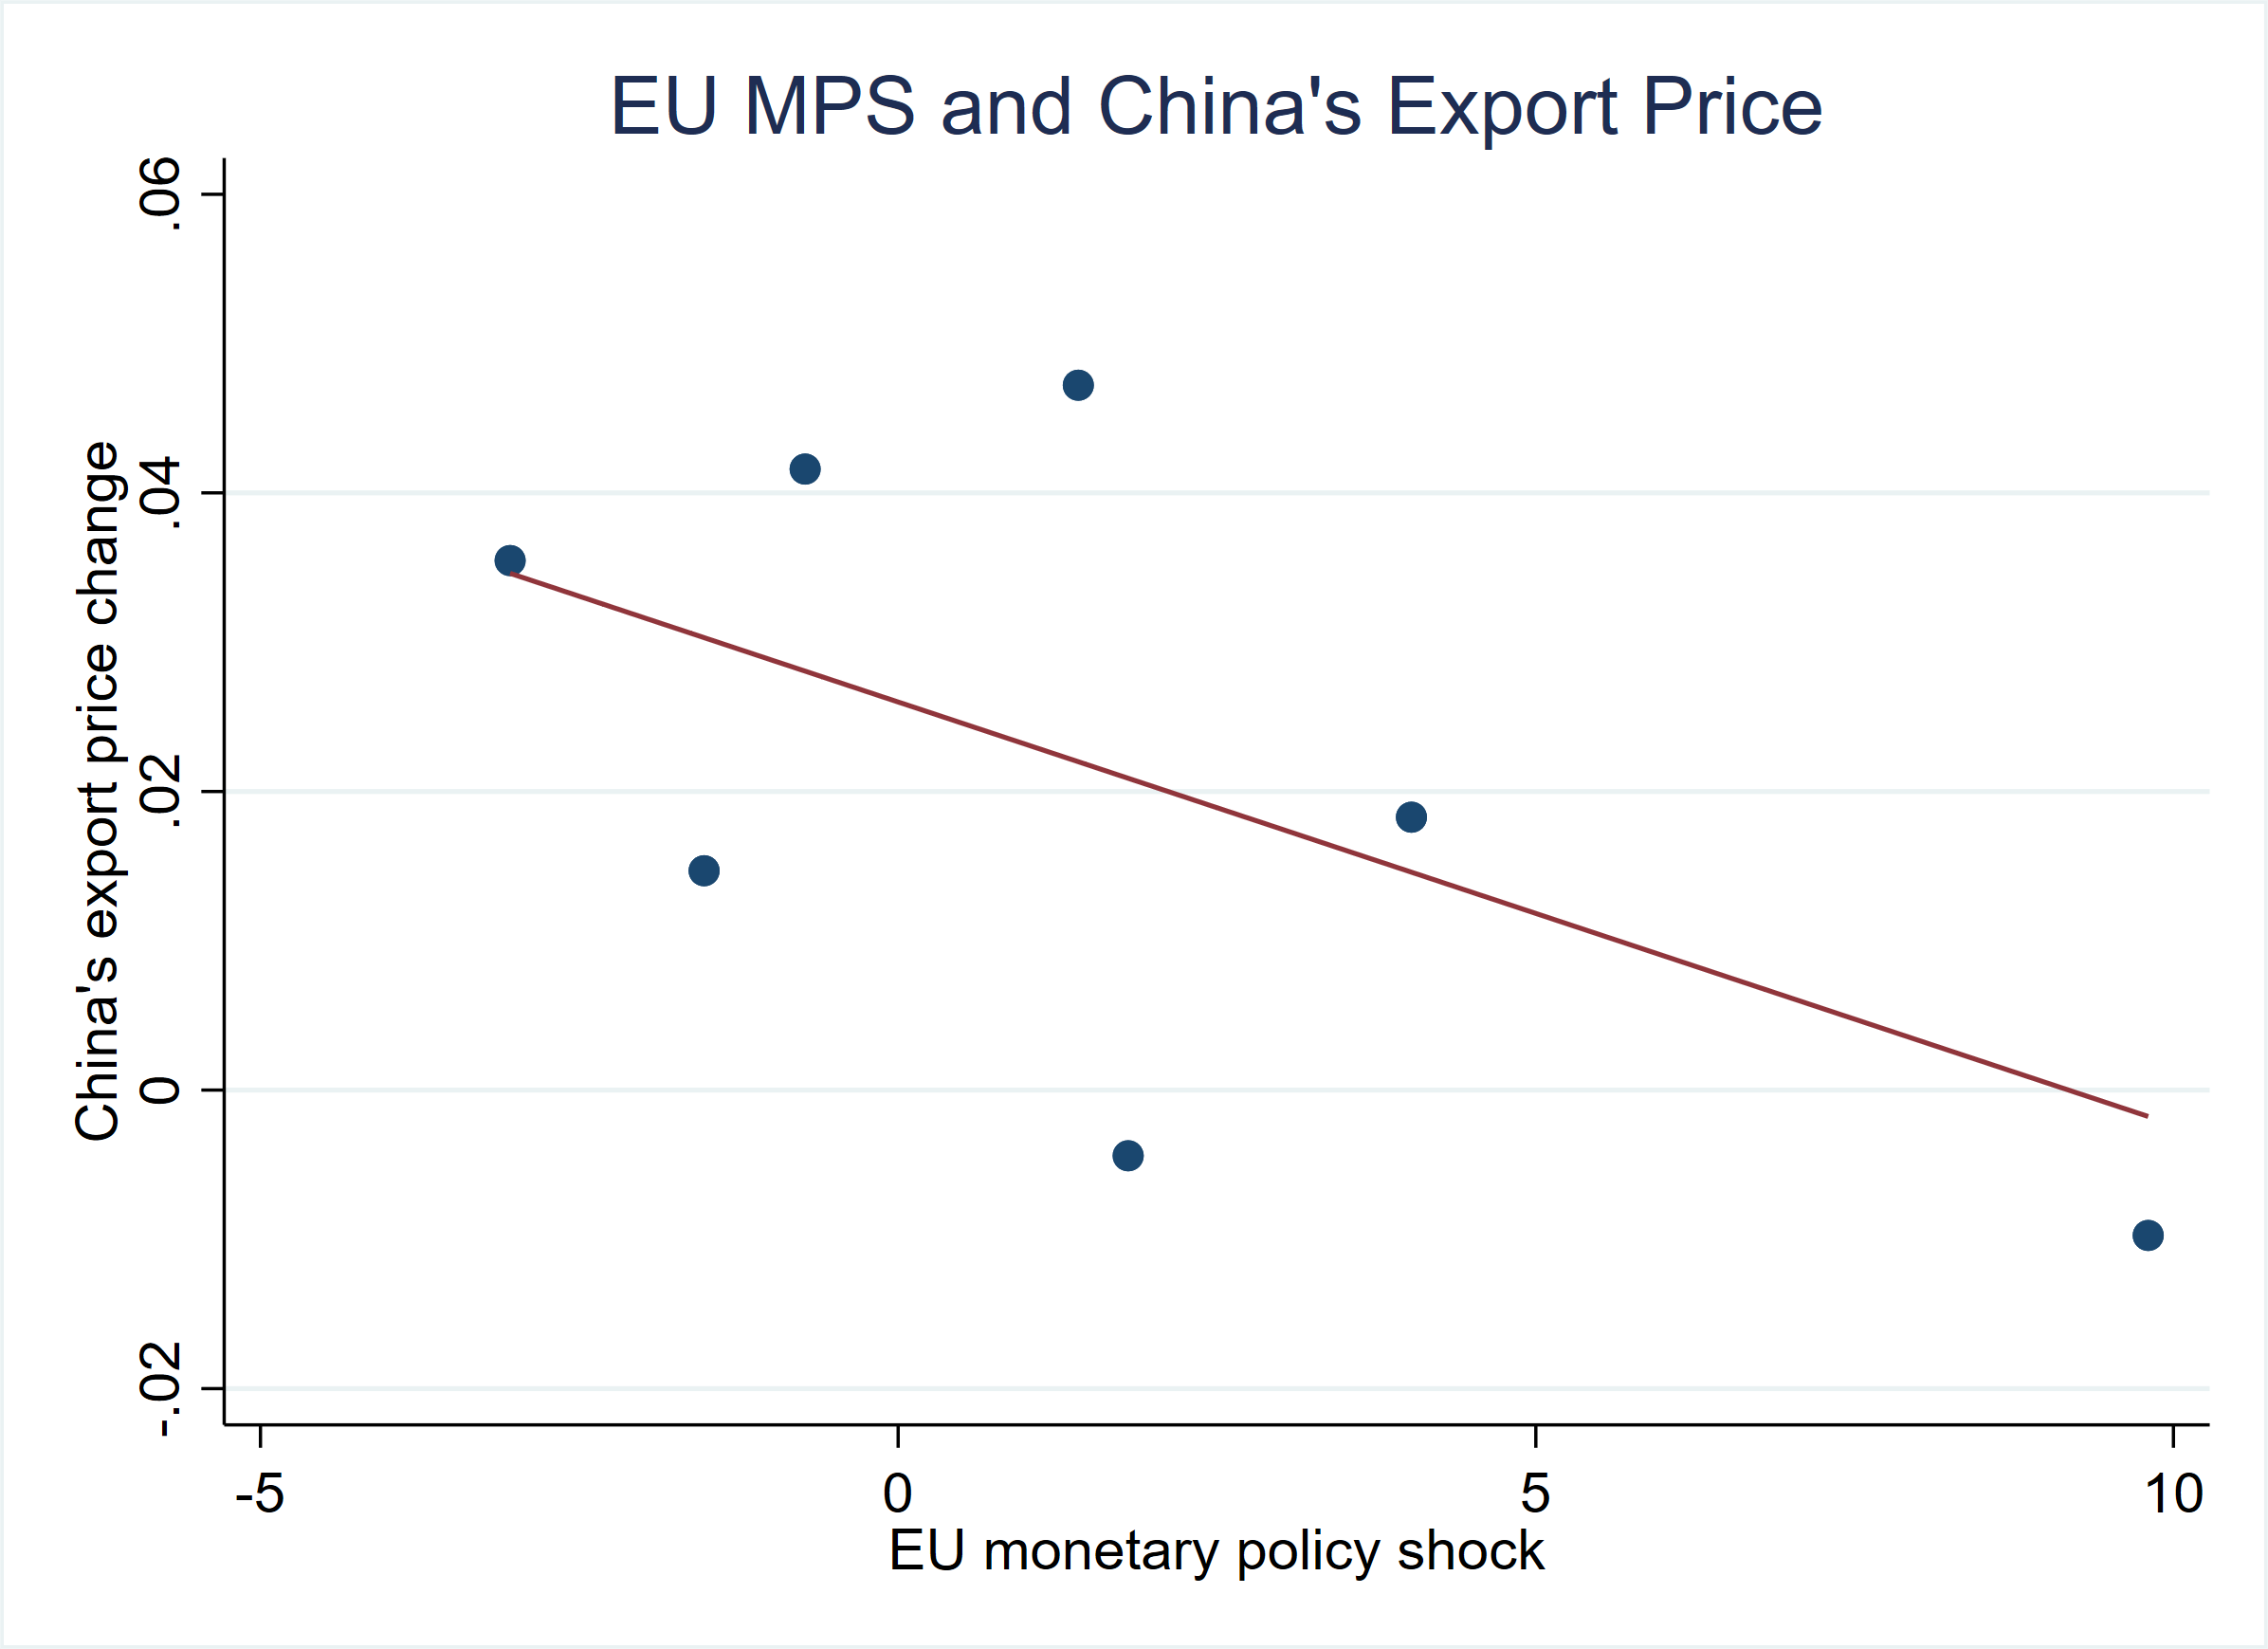
\includegraphics[width=\columnwidth]{latex/slides/pic_Jun2023/EU_shock.png}
    		\label{fig.EU_shock}
    	\end{figure}
        \end{columns}
        \item However, the UK and Japan monetary policy shocks have no significant effect on China's export price.
    \end{itemize}
\end{frame}

\begin{frame}{Baseline Results: US Shocks}
    \begin{itemize}
        \item A one-unit tightening shock (2Y US treasury yield increases by 100 basis points) implies that the average export price increases by 0.13 percentage points in the same year while the average export quantity decreases by 1.6 percentage points in the next year.
    \end{itemize}
    \begin{table}[htbp]
        \centering  
        \vspace{-5mm}
        \caption{Effect of U.S. monetary policy shocks on Chinese export prices and quantities}
        \resizebox{0.75\columnwidth}{!}{
        \begin{threeparttable}
            \begin{tabular}{lccccc}
                \toprule
                      & (1)   & (2)   & (3)   & (4)   & (5) \\
                \midrule
                    Dependent variable:  & \multicolumn{3}{c}{ $\Delta ln(price)_{ijct}$} & \multicolumn{2}{c}{ $\Delta ln(quantity)_{ijct}$}\\
                \midrule
                $brw_{t}$   & 0.133*** & 0.131*** &       & -0.892 &  \\
                      & (0.025) & (0.025) &       & (0.600) &  \\
                $brw_{t-1}$ & &       & 0.059 &       & -1.601** \\
                      &  &  & (0.033) &       & (0.447) \\
                $\Delta ln(RER)_{ct}$ &  & 0.050** & 0.100** & -0.022 & -1.081* \\
                      & (0.020) & (0.035) & (0.665) & (0.543) \\
                $\Delta ln(RGDP)_{ct}$ & 0.271** & 0.282** & 0.468*** & -1.860 & -2.918* \\
                & (0.104) & (0.103) & (0.088) & (1.714) & (1.341) \\
                Fixed effects   &  \multicolumn{5}{c}{Firm-product–country fixed effects} \\   
                Observations    & 1080269 & 1080269 & 1080269 & 1076863 & 1076863 \\
                \bottomrule
            \end{tabular}
            \begin{tablenotes}
                \footnotesize
                \item Notes: Robust standard errors clustered at firm-product-country level and year level;  *, **, and *** indicate significance at 10\%, 5\%, and 1\% levels; All regressions include a constant term and firm-product-country level fixed effects.
            \end{tablenotes}
        \end{threeparttable}
        }
	\label{tab.baseline}
    \end{table}
\end{frame}

\begin{frame}{Compared with EU Shocks}
    \begin{table}[htbp]
        \centering  
        \vspace{-5mm}
        \caption{Effect of EU monetary policy shocks on Chinese export prices and quantities}
        \resizebox{0.75\columnwidth}{!}{
        \begin{threeparttable}
            \begin{tabular}{lccccc}
                \toprule
                      & (1)   & (2)   & (3)   & (4)   & (5) \\
                \midrule
                    Dependent variable:  & \multicolumn{3}{c}{ $\Delta ln(price)_{ijct}$} & \multicolumn{2}{c}{ $\Delta ln(quantity)_{ijct}$}\\
                \midrule
                $target_t$ & -0.003** & -0.003** &       & 0.051** &  \\
                & (0.001) & (0.001) &       & (0.017) &  \\
                $path_t$ & -0.001 & -0.000 &       & -0.009 &  \\
                & (0.002) & (0.003) &       & (0.032) &  \\
                $target_{t-1}$ &       &       & -0.001 &       & 0.008 \\
                &       &       & (0.001) &       & (0.013) \\
                $path_{t-1}$ &       &       & -0.004 &       & 0.054 \\
                &       &       & (0.003) &       & (0.036) \\
                $\Delta ln(RER)_{ct}$ &       & 0.071 & 0.069 & -0.349 & 0.062 \\
                &       & (0.037) & (0.040) & (0.681) & (0.404) \\
                $\Delta ln(RGDP)_{ct}$ & 0.325** & 0.323** & 0.290** & 0.106 & -0.524 \\
                & (0.128) & (0.131) & (0.109) & (1.150) & (1.644) \\
                Fixed effects   &  \multicolumn{5}{c}{Firm-product–country fixed effects} \\   
                Observations    & 1080269 & 1080269 & 1080269 & 1076863 & 1076863 \\
                \bottomrule
            \end{tabular}
            \begin{tablenotes}
                \footnotesize
                \item Notes: Robust standard errors clustered at firm-product-country level and year level;  *, **, and *** indicate significance at 10\%, 5\%, and 1\% levels; All regressions include a constant term and firm-product-country level fixed effects.
            \end{tablenotes}
        \end{threeparttable}
        }
	\label{tab.baseline}
    \end{table}
\end{frame}

\begin{frame}{Firm Heterogeneity}
    \begin{itemize}
        \item Next, we introduce interaction terms $EXP_{jt}$ to test whether heterogeneity in firms' exposure to monetary policy shocks affects the degree of markups.
        \begin{equation}
    	\Delta \ln P_{i j c t}=\beta_1 M P_{t}^{US} + \beta_2 (M P_{t}^{US} \times EXP_{jt})+ \mathbf{Z}_{jt} \boldsymbol{\gamma}^{\prime}+\mathbf{X}_{ct} \boldsymbol{\delta}^{\prime} +\xi_{i j c} + \varepsilon_{ijct}
    	\label{eq.exposure}
        \end{equation}
        \item Firm-level heterogeneous exposure to financial shocks $EXP_{jt}$ includes firm size, import status, import intensity, interest expense to sales ratio, etc.
        \item The import intensity of a firm is defined as the ratio of total import value over its total variable costs (as in \cite{aik2014}):
        $$\varphi_{jt} \equiv \frac{\text{Total import value}_{jt}}{\text{Intermediate input}_{jt}+\text{Wage payment}_{jt}}$$
    \end{itemize}
\end{frame}

\begin{frame}{Firm Heterogeneity}
    \begin{table}[htbp]
        \centering  
        \vspace{-5mm}
        \caption{Firm Heterogeneity in firm size and import intensity}
        \resizebox{0.7\columnwidth}{!}{
        \begin{threeparttable}
            \begin{tabular}{lcccc}
                \toprule
                      & (1)   & (2)   & (3)   & (4) \\
                \midrule
                      & \multicolumn{4}{c}{Dependent variable: $\Delta ln(price)_{ijct}$} \\
                \midrule
                $brw_t$   & -0.045 & 0.174*** & 0.134*** & 0.116*** \\
                      & (0.071) & (0.027) & (0.027) & (0.021) \\
                $brw_t\times Sales_{jt}$ & 0.015** &       &       &  \\
                      & (0.006) &       &       &  \\
                $brw_t\times Twoway_{jt}$ &       & -0.055** &       &  \\
                      &      & (0.022) &       &  \\
                $brw_t\times \mathbf{1}\{\varphi_{jt}\geq\varphi_{jt}^{Q3}\}$ &     &       & -0.016 &  \\
                      &      &       & (0.018) &  \\
                $brw_t\times \mathbf{1}\{(I/S)_{jt}\geq (I/S)_{jt}^{Q3}\}$ &       &       & & 0.057** \\
                      &       &       & & (0.017) \\
                $\Delta ln(RER)_{ct}$ & 0.055* & 0.055* & 0.055* & 0.055* \\
                      & (0.024) & (0.024) & (0.024) & (0.024) \\
                $\Delta ln(RGDP)_{ct}$ & 0.289** & 0.294** & 0.287** & 0.289** \\
                      & (0.108) & (0.107) & (0.105) & (0.106) \\
            Observations    & 1080193 & 1080193 & 1080193 & 1080193 \\
                \bottomrule
            \end{tabular}
            \begin{tablenotes}
                \footnotesize
                \item Notes: Robust standard errors clustered at firm-product-country level and year level;  *, **, and *** indicate significance at 10\%, 5\%, and 1\% levels; All regressions include a constant term and firm-product-country level fixed effects.
            \end{tablenotes}
        \end{threeparttable}
        }
	\label{tab.baseline}
    \end{table}
\end{frame}

\begin{frame}{Country Heterogeneity}
    \begin{itemize}
        \item We find the price response to US monetary policy shocks is not significant for the export to the US, but it is significant for exports to other country groups.
    \end{itemize}
    \begin{table}[htbp]
        \centering  
        \vspace{-5mm}
        \caption{Export price to different destination countries}
        \resizebox{0.75\columnwidth}{!}{
        \begin{threeparttable}
            \begin{tabular}{lccccc}
                \toprule
                      &  US & Non-US & EU & OECD & Emerging\\
                      & (1)   & (2)   & (3)   & (4)   & (5) \\
                \midrule
                      & \multicolumn{5}{c}{Dependent variable: $\Delta ln(price)_{ijct}$} \\
                \midrule
                $brw_{t}$   & 0.026 & 0.142*** & 0.151*** & 0.136*** & 0.160*** \\
                      & (0.044) & (0.024) & (0.022) & (0.023) & (0.029) \\ \\
                $\Delta ln(RER)_{ct}$ & -0.202* & 0.057** & 0.086* & 0.063* & 0.025 \\
                      & (0.101) & (0.022) & (0.041) & (0.031) & (0.025) \\
                $\Delta ln(RGDP)_{ct}$ & 0.950 & 0.285** & 0.921*** & 0.497*** & 0.070 \\
                & (0.504) & (0.111) & (0.181) & (0.102) & (0.157) \\
                Fixed effects   &  \multicolumn{5}{c}{Firm-product–country fixed effects} \\   
                Observations    & 114489 & 965280 & 209584 & 705928 & 182154 \\
                \bottomrule
            \end{tabular}
            \begin{tablenotes}
                \footnotesize
                \item Notes: Robust standard errors clustered at firm-product-country level and year level;  *, **, and *** indicate significance at 10\%, 5\%, and 1\% levels; All regressions include a constant term and firm-product-country level fixed effects.
            \end{tablenotes}
        \end{threeparttable}
        }
	\label{tab.country}
    \end{table}
\end{frame}

\begin{frame}{Decomposition of Price: Markup vs. Marginal Cost}
    \begin{itemize}
        \item Since we do not know the input of each exported product, we follow the method of \cite{dlw2012} to derive the firm-specific markup as the ratio of the factor’s output elasticities to its firm-specific factor payment shares $\mu_{jt}=\theta_{jt}^{X}/\alpha_{jt}^{X}$.
        \item Therefore, the marginal cost of production is estimated as the unit value over the firm-level markup: $MC_{ijct}=P_{ijct}/\mu_{jt}$.
        \item We conduct firm-level and transaction-level regressions of markups and marginal costs on monetary policy shocks.
        \begin{equation}
            \Delta \ln MC_{ijct}=\beta^{mc} M P_{t} + \mathbf{Z}_{jt} \boldsymbol{\gamma}^{\prime}+\mathbf{X}_{ct} \boldsymbol{\delta}^{\prime} +\xi_{i j c} + \varepsilon_{ijct}
    	\label{eq.mc}
        \end{equation}
    \end{itemize}
\end{frame}

\begin{frame}{Decomposition of Price: Markup vs. Marginal Cost}
    \begin{itemize}
        \item By decomposition of price, most price responses are from changes in production cost rather than firm-level markup.
    \end{itemize}
    \begin{table}[htbp]
        \centering  
        \vspace{-5mm}
        \caption{Decomposition of Price: Markup vs. Marginal Cost}
        \resizebox{0.65\columnwidth}{!}{
        \begin{threeparttable}
            \begin{tabular}{lcccc}
                \toprule
                      & (1)   & (2)   & (3)   & (4)  \\
                \midrule
                    Dependent variable:  & $\Delta ln(MC)_{ijct}$ &\multicolumn{3}{c}{ $\Delta ln(price)_{ijct}$} \\
                \cmidrule{2-2} \cmidrule{3-5}
                $brw_{t}$ & 0.166*** & -0.013 & 0.138*** & 0.138*** \\
                    & (0.029) & (0.013) & (0.030) & (0.030) \\
                & (0.150) & (0.059) & (0.121) & (0.121) \\
                $\Delta ln(MC)_{ijct}$ &       & 0.902*** &       &  \\
                &       & (0.006) &       &  \\
                $\Delta Markup_{jt}$ &       &       & 0.011** & 0.005 \\
                &       &       & (0.003) & (0.004) \\
                $Markup_{jt-1}$ &       &       &       & -0.011* \\
                &       &       &       & (0.005) \\
                $\Delta ln(RER)_{ct}$ & 0.040 & 0.017 & 0.050* & 0.050* \\
                & (0.027) & (0.021) & (0.025) & (0.026) \\
                $\Delta ln(RGDP)_{ct}$ & 0.278 & 0.042 & 0.314** & 0.316** \\
                Fixed effects   &  \multicolumn{4}{c}{Firm-product–country fixed effects} \\   
                Observations    & 773784 & 772230 & 770114 & 770114\\
                \bottomrule
            \end{tabular}
            \begin{tablenotes}
                \footnotesize
                \item Notes: Robust standard errors clustered at firm-product-country level and year level;  *, **, and *** indicate significance at 10\%, 5\%, and 1\% levels; All regressions include a constant term and firm-product-country level fixed effects.
            \end{tablenotes}
        \end{threeparttable}
        }
	\label{tab.markup}
    \end{table}
\end{frame}

\begin{frame}{Further Decomposition of Production Cost}
    \begin{itemize}
        \item A tightening monetary policy shock will reduce firms' trade credit provision, increase financial and interest expenses, and reduce the average wages.
        \begin{equation}
            \Delta \ln Cost_{jt}=\beta^{cost} M P_{t} + \mathbf{Z}_{jt} \boldsymbol{\gamma}^{\prime} +\xi_{j} + \varepsilon_{jt}
    	\label{eq.mc}
        \end{equation}
    \end{itemize}
        \begin{table}[htbp]
        \centering  
        \vspace{-5mm}
        \caption{Effect of US monetary policy shocks on firm-level cost variables}
        \resizebox{0.85\columnwidth}{!}{
        \begin{threeparttable}
            \begin{tabular}{lcccc}
                \toprule
                      & (1)   & (2)   & (3)   & (4)  \\
                \midrule
                    Dependent variable:  & $\Delta (Arec/Sales)_{jt}$ & $\Delta (FE/ L)_{jt}$ & $\Delta (IE/L)_{jt}$ & $\Delta ln(Wage)_{jt}$\\
                \midrule
                $brw_{t}$ & -0.010*** & 0.002*** & 0.002*** & -0.079*** \\
                    & (0.001) & (0.001) & (0.000) & (0.005) \\
                $ln(Sales)_{jt-1}$ & 0.033*** & -0.002*** & -0.001*** & -0.035*** \\
                & (0.000) & (0.000) & (0.000) & (0.001) \\
                Fixed effects   &  \multicolumn{4}{c}{Firm fixed effects} \\   
                Observations    & 885626 & 877233 & 877088 & 882351 \\
                \bottomrule
            \end{tabular}
            \begin{tablenotes}
                \footnotesize
                \item Notes: Robust standard errors clustered at the firm level;  *, **, and *** indicate significance at 10\%, 5\%, and 1\% levels; All regressions include a constant term and firm-level fixed effects.
            \end{tablenotes}
        \end{threeparttable}
        }
	\label{tab.interest}
    \end{table}
\end{frame}

\begin{frame}{Robustness Check}
    \begin{enumerate}
        \item use alternative measures of monetary policy shocks; 
        \item use alternative measures of price changes: product-level and firm-level price index;
        \item use alternative denominated currencies: local currency pricing (LCP) vs dominant currency pricing (DCP) vs vehicle currency pricing (VCP);
        \item use alternative periods: pegged exchange rate regime vs floating exchange rate regime, zero-lower-bound (ZLB) VS non-zero-lower-bound (non-ZLB);
        \item control other cost-push shocks (e.g. oil news shock);
        \item construct time-invariant firm-level interaction terms $EXP_j$ to deal with the contemporaneous endogeneity
    \end{enumerate}
\end{frame}

%%%%%%%%%%%%%%%%%%%%%%%%%%%%%%%%%%%%%%%%%%%%%%%%%%
\section{Model}

\begin{frame}{Conceptual framework}
\begin{itemize}
    \item Imagine a three-country world: US, China, South Korea; 
    \item Now there is a contractionary monetary shock from the US, how South Korea is affected? 
    \item Demand side (directly from US): R (+), Y (-), P(-).
    \item Supply side (indirectly from China): Cost (+), Y (-), P(+).
    \item \textbf{Summary}: China aggravates the impact of US shock on South Korea  
\end{itemize}
        \begin{figure}[htbp]
		\centering 
        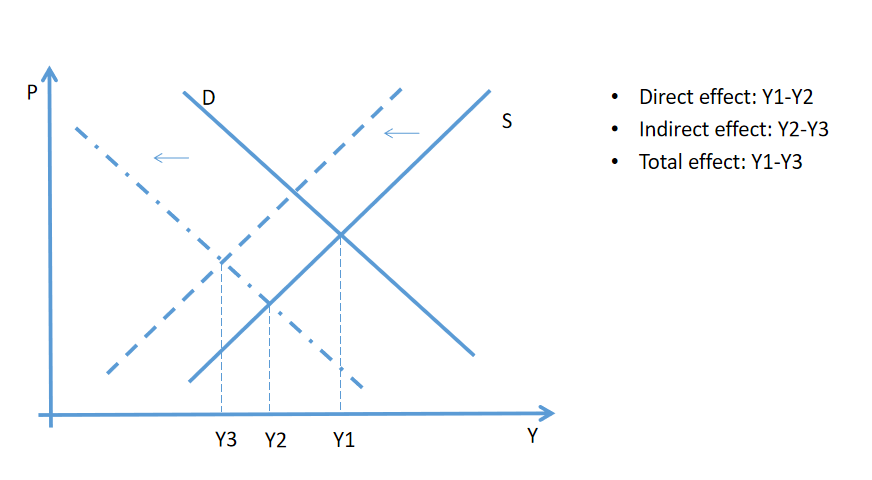
\includegraphics[width=0.8\columnwidth]{latex/slides/pic_Jun2023/DS_curve.png}
		\label{DS_curve}
	\end{figure}  
\end{frame}

\begin{frame}{Households}
\fontsize{8}{8}\selectfont

\begin{itemize}
    \item A home country (China) consumer receives utility from consumption, $C_{t}$, and disutility from labor, $L_{t}$. Its lifetime utility is
\end{itemize}


$$
V_{t}=\max \mathbb{E}_{t} \sum_{j=0}^{\infty} \beta^{j}\left[\frac{C_{t+j}{ }^{1-\sigma}-1}{1-\sigma}-\psi \frac{L_{t+j}^{1+\chi}}{1+\chi}\right]
$$

\begin{itemize}
    \item where $\beta \in(0,1)$ is the discount factor, $\sigma>0$ is the inverse elasticity of intertemporal substitution, $\chi \geq 0$ is the inverse Frisch elasticity, and $\psi>0$ is a scaling parameter. The saver's budget constraint is:
\end{itemize}


$$
P_{t} C_{t}+S_{t}+\mathbb{E}_{t} \Lambda_{t, t+1} \mathcal{D}_{t+1} \leq W_{t} L_{t}+R_{t-1} S_{t-1}+\mathcal{D}_{t}+P_{t} D_{t}+P_{t} T_{t}
$$



\begin{itemize}
    \item The consumer earns nominal income from labor, with a wage of $W_{t}$, receives dividends from ownership in firms, $D_{t}$, and receives a lump-sum transfer from the fiscal authority, $T_{t}$. It can save via a one-period deposit, $S_{t}$, that pays gross nominal interest rate, $R_{t}$. The consumption index is a composition of home and foreign goods, so
\end{itemize}



$$
C_{t}\equiv\left(C_{H, t}\right)^{1-\gamma}\left(C_{F, t}\right)^{\gamma}
$$

\begin{itemize}
    \item and the corresponding CPI $P_{t}$ can be expressed as
\end{itemize}

$$
P_{t}=k^{-1} P_{H, t}^{1-\gamma} P_{F, t}^{\gamma}, \ where \ k \equiv(1-\gamma)^{(1-\gamma)} \gamma^{\gamma}
$$

\end{frame}

\begin{frame}{Households (continued)}
\fontsize{8}{8}\selectfont

\begin{itemize}
    \item Since the prices are set in the producer currency, law of one price holds. We will have $P_{F, t}=P_{F, t}^{*} \mathcal{E}_{t}$ and $P_{H, t}^{*}=\frac{P_{H, t}}{\mathcal{E}_{t}}$, where $\mathcal{E}_{t}$ is the nominal exchange rate, defined as the price of foreign currency in terms of domestic currency. 
\end{itemize}


$$
\mathcal{E}_{t}=\frac{P_{t}}{P_{t}^{*}}
$$



\begin{itemize}
    \item The terms of trade is then given by
\end{itemize}


$$
\mathcal{T}_{t} \equiv \frac{P_{F, t}}{P_{H, t}}=\frac{P_{F, t}^{*} \mathcal{E}_{t}}{P_{H, t}}
$$

\begin{itemize}
    \item The first-order conditions for consumption allocation, labor supply and intertemporal optimization are
\end{itemize}



$$
\begin{aligned}
& P_{H, t} C_{H, t}=(1-\gamma) P_{t} C_{t} \\
& P_{F, t} C_{F, t}=\gamma P_{t} C_{t} \\
& \beta\left(C_{t} / C_{t-1}\right)^{-\sigma}\left(P_{t-1} / P_{t}\right)=\Lambda_{t-1, t} \\
& 1 / R_{t}=\mathbb{E}_{t} \Lambda_{t, t+1} \\
& \frac{W_{t}}{P_{t}\left(C_{t}\right)^{\sigma}}=\psi L_{t}^{\chi}
\end{aligned}
$$
\end{frame}

\begin{frame}{Producer-final goods}

\begin{itemize}
    \item Each final goods firm in the home country uses a continuum of intermediate goods to produce output, according to the following CES technology:
\end{itemize}


$$
Y_{t}=\left(\int_{0}^{1} Y_{t}(f)^{(\epsilon-1) / \epsilon} \mathrm{d} f\right)^{\epsilon /(\epsilon-1)}
$$

\begin{itemize}
    \item where $Y_{t}$ denotes aggregate output, while $Y_{t}(f)$ is the input produced by intermediate goods firm $f$. Both variables are normalized by population size $1-\gamma$, i.e., they are expressed in per capita terms. Profit maximization, taking the price of the final good $P_{\mathrm{H}, t}$ as given, implies the set of demand equations:
\end{itemize}

$$
Y_{t}(f)=\left(\frac{P_{\mathrm{H}, t}(f)}{P_{\mathrm{H}, t}}\right)^{-\epsilon} Y_{t}
$$

\begin{itemize}
    \item as well as the domestic price index
\end{itemize}


$$
P_{\mathrm{H}, t}=\left(\int_{0}^{1} P_{\mathrm{H}, t}(f)^{1-\epsilon} \mathrm{d} f\right)^{1 /(1-\epsilon)}
$$

\end{frame}

\begin{frame}{Producer-intermediate goods}

\fontsize{8}{8}\selectfont

\begin{itemize}
    \item Each intermediate firm $f$ in the home economy has the following production technology.
\end{itemize}

$$
Y_{t}(f)=A_{t} L_{t}(f)
$$

\begin{itemize}
    \item where $A_{t}$ is an exogenous country-specific productivity disturbance obeying a known stochastic process. Following Ravenna and Walsh (2006, JME). We assume The firm must borrow an amount $W_tL_t(f)$ from intermediaries at the gross nominal interest rate $R_t$, so the nominal cost of labor is $R_tW_t$. The real marginal cost is the same for all firms. This implies the minimized nominal marginal cost of production is
\end{itemize}

$$
M C_{t}(f)=\frac{w_{t} P_{t}R_{t}}{A_{t}}
$$

\begin{itemize}
    \item where $w_{t}=\frac{W_{t}}{P_{t}}$ is the real wage.
\end{itemize}


\begin{itemize}
    \item Export prices are assumed to be set in producer currency (PCP). Intermediate firms are subject to a Calvo (1983) pricing friction in each period, firm $f$ resets its prices with probability $1-\phi$, with $\phi \in[0,1]$.
\end{itemize}

$$
\max _{\tilde{P}_{H, t}(f)} \mathbb{E}_{t} \sum_{j=0}^{\infty} \phi^{j} \Lambda_{t, t+j}^{s}\left[\left(1-\tau_{H}\right)\left(\frac{\tilde{P}_{H, t}(f)}{P_{H, t+j}}\right)^{-\epsilon} Y_{t+j} \tilde{P}_{H, t}(f)-\left(\frac{\tilde{P}_{H, t}(f)}{P_{H, t+j}}\right)^{-\epsilon} Y_{t+j} M C_{t+j}(f)\right]
$$

\begin{itemize}
    \item where $\tau_{H}=\frac{1}{\phi-1}$ is a subsidy imposed by the government to eliminate the steady state monopolistic distortion.
\end{itemize}

\end{frame}

\begin{frame}{Producer-intermediate goods (continued)}

\begin{itemize}
    \item With the symmetric assumption, $\tilde{P}_{H, t}(f)=\tilde{P}_{H, t}$. The optimal reset price satisfies:
\end{itemize}


$$
\begin{aligned}
\tilde{P}_{H, t} & =\frac{\epsilon}{\epsilon-1} \frac{X_{1, t}}{X_{2, t}} \\
X_{1, t} & =P_{H, t}^{\epsilon} M C_{t} Y_{t}+\phi \mathbb{E}_{t} \Lambda_{t, t+1} X_{1, t+1} \\
X_{2, t} & =P_{H, t}^{\epsilon} Y_{t}+\phi \mathbb{E}_{t} \Lambda_{t, t+1} X_{2, t+1}
\end{aligned}
$$

\begin{itemize}
    \item Due to the law of large numbers, the price level satisfies:
\end{itemize}

$$
\left(P_{H, t}\right)^{1-\epsilon}=\phi\left(P_{H, t-1}\right)^{1-\epsilon}+(1-\phi)\left(\tilde{P}_{H, t}\right)^{1-\epsilon}
$$

\end{frame}

\begin{frame}{Financial intermediary}
    
\begin{itemize}
    \item The financial intermediary receives household deposits and a cash injection $X_t$ from the monetary authority. These funds are lent to firms at a gross nominal interest rate of $R_t$.
\end{itemize}

\begin{itemize}
    \item  Intermediaries operate costlessly in a competitive environment, so profits in the intermediary industry are 
\end{itemize}

$$
\Pi_t=R_t(S_t+X_t)-R_tS_t=X_t
$$

\begin{itemize}
    \item Equilibrium in the market for loans implies that 
\end{itemize}

$$
W_tL_t=S_t+X_t
$$ 

\begin{itemize}
    \item where $L_t$ is aggregate labor demand by firms
\end{itemize}


\end{frame}

\begin{frame}{Shocks}

\begin{itemize}
    \item It is assumed that the productivity shocks $\left(A_{t}\right)$ obey stationary $A R(1)$ processes, where the non-stochastic steady state value of productivity is normalized to unity.
\end{itemize}
$$
\begin{gathered}
\ln A_{t}=\rho_{A} \ln A_{t-1}+s_{A} \varepsilon_{A, t}
\end{gathered}
$$

\begin{itemize}
    \item The Taylor rule of the central bank's policy rate follows the following process:
\end{itemize}
\begin{gather*}
\ln R_{t}=\left(1-\rho_{r}\right) \ln R +\rho_{r}\ln R_{t-1} + \left(1-\rho_{r}\right) [ \phi_{\pi}\left(\ln \Pi_{t}-\ln \Pi\right)+ \\ 
\phi_{x}\ln Y_{t}-\ln Y_{t}^{N} ] +s_{r}\varepsilon_{r,t}+s_{g}^{H}\varepsilon_{g, t}
\end{gather*}

\begin{itemize}
    \item where $\varepsilon_{g, t}$  is the global monetary monetary policy shock and $s_{g}^{H}$ is the corresponding responding coefficient. All the shocks are assumed to be IID.
\end{itemize}

\begin{itemize}
    \item For the foreign central bank:
\end{itemize}
\begin{gather*}
\ln R_{t}^{*}=\left(1-\rho_{r}^{*}\right) \ln R^{*}+ \rho_{r}^{*}\ln R_{t-1}^{*} + \left(1-\rho_{r}^{*}\right)[\phi_{\pi}^{*}\left(\ln \Pi_{t}^{*}-\ln \Pi^{*}\right)+ \\ \phi_{x}^{*}\ln Y_{t}^{*}-\ln Y_{t}^{N*}] 
 +s_{r}^{*}\varepsilon_{r, t}+s_{g}^{F}\varepsilon_{g, t}
\end{gather*}

\end{frame}

\begin{frame}{Aggregation}

\begin{itemize}
    \item Goods market clearing conditions for 
     the home and foreign countries are
\end{itemize}
\begin{gather*}
(1-\gamma) Y_{t}=(1-\gamma)C_{H, t}+\gamma C_{H, t}^{*} \\
\gamma Y_{t}^{*}=(1-\gamma)C_{F, t}+\gamma C_{F, t}^{*}
\end{gather*}
\begin{itemize}
    \item Then we obtain
\end{itemize}
\begin{gather*}
P_{H, t} Y_{t}=(1-\gamma)P_{t}C_{t}+\gamma P_{t}C_{t}^{*} \\
P_{F, t} Y_{t}^{*}=(1-\gamma) P_{t}C_{t}+\gamma P_{t}C_{t}^{*} \\
\frac{P_{H, t}}{P_{F, t}}=\frac{Y_{t}^{*}}{Y_{t}}
\end{gather*}

\end{frame}

\begin{frame}{Aggregation (continued)}

\begin{itemize}
    \item If we assume that initial net international asset holding is 0, then the trade balance is zero:
\end{itemize}


$$
\begin{aligned}
P_{H, t} Y_{t} & =P_{t}C_{t} \\
P_{F, t}^{*} Y_{t}^{*} & =P_{t}^{*}C_{t} .
\end{aligned}
$$

\begin{itemize}
    \item Zero trade balance condition and Equation also imply complete risk sharing between home and foreign countries:
\end{itemize}


$$
C_{t}=C_{t}^{*}
$$

\begin{itemize}
    \item We can also get
\end{itemize}


$$
Y_{t}=\frac{P_{t}}{P_{H, t}}C_{t}=k^{-1}C_{t} \mathcal{T}_{t}^{\gamma}
$$

\begin{itemize}
    \item where the second equality is from price index Equation and definition of $\mathcal{T}_t$ (terms of trade).  
\end{itemize}
  
\end{frame}

\begin{frame}{Aggregation (continued)}

\begin{itemize}
    \item On the supply side,
\end{itemize}

$$
Y_{t}=\frac{A_{t} L_{t}}{V_{t}}
$$

$$
V_{t} \equiv \int_{0}^{1}\left(\frac{P_{H, t}(f)}{P_{H, t}}\right)^{-\epsilon} d f \geq 1
$$

$$
\mathcal{T}_{t}=\frac{Y_{t}}{Y_{t}^{*}}
$$

\begin{itemize}
    \item Combining the labor supply and demand, and then using the aggregate demand and the aggregate production, yields the real marginal cost (in terms of the home producer index):
\end{itemize}


$$
\begin{aligned}
m c_{t} & =w_{t}R_{t} / A_{t} \\
& =\psi\left(k Y_{t}^{1-\gamma}\left(Y_{t}^{*}\right)^{\gamma}-C_{t}^{b}\right)^{\sigma} Y_{t}^{\chi+\gamma} A_{t}^{-\chi} V_{t}^{\chi}R_{t}
\end{aligned}
$$  
\end{frame}
    
\begin{frame}{Linear model}

\begin{itemize}
    \item The IS curve for home country is
\end{itemize}


$$
x_{t}= \mathbb{E}_{t} x_{t+1}-\frac{1}{\sigma_{0}}\left(r_{t}-\mathbb{E}_{t} \pi_{t+1}-r_t^N\right)
$$
$$
r_{t}^{N}=\sigma_{0} \mathbb{E}_{t} \Delta y_{t+1}^{N}+\kappa_{0} y_{t+1}^{*}
$$
\begin{itemize}
    \item The Phillips curve for home-produced goods is
\end{itemize}

$$
\pi_{H, t}=\nu\left[\varkappa y_{t}-(1+\chi) a_{t}+\kappa_{0}y_{t}^{*}+\textcolor{blue}{r_t}\right]+\beta \mathbb{E}_{t} \pi_{H, t+1}
$$

\begin{itemize}
    \item Or
\end{itemize}

$$
\pi_{H, t} =\nu \varkappa\left(y_{t}-y_{t}^{N}\right)+\textcolor{blue}{\nu(r_t-r_t^N)}+\beta \mathbb{E}_{t} \pi_{H, t+1}
$$

\begin{itemize}
    \item where $\nu=\frac{(1-\phi)(1-\phi \beta)}{\phi}$, $\sigma_0=\sigma-\kappa_{0}$, $\varkappa=\chi+\sigma-\kappa_{0}$ and $\kappa_{0}=\sigma \gamma-\gamma$. Lowercase variables with a $t$ subscript denote $\log$ deviations from the non-stochastic steady state. $y_{t}$ and $y_{t}^{*}$ are the output of home and foreign countries, and $\pi_{H, t}$ and $\pi_{F, t}$ are home and foreign PPI inflation. $r_{t}$ and $r_{t}^{*}$ are the short-term nominal interest rates.
\end{itemize}

\end{frame}

\begin{frame}{Linear model (continued)}

\begin{itemize}
    \item We can define $y_{t}^{N}$ and $y_{t}^{N *}$ as the equilibrium level of output consistent with price flexibility in the domestic country while taking foreign output as exogenously given:
\end{itemize}

$$
\begin{gathered}
y_{t}^{N}=\varkappa^{-1}\left[(1+\chi) a_{t}-\kappa_{0} y_{t}^{*}\right], \\
y_{t}^{N *}=\varkappa^{*-1}\left[(1+\chi) a_{t}^{*}-\kappa_{0}^{*} y_{t}\right] .
\end{gathered}
$$



\begin{itemize}
    \item where $\kappa_{0}=\sigma \gamma-\gamma$. And $r_{t}^{N}$ and $r_{t}^{N *}$ are the natural rates of interest of the two countries.
\end{itemize}

\begin{itemize}
    \item Terms of trade is the difference of output gap between two countries plus the natural level of terms of trade:
\end{itemize}


$$
\tau_{t}=y_{t}-y_{t}^{*}
$$
\begin{itemize}
    \item The model is closed by monetary policy.
\end{itemize}

\end{frame}


\begin{frame}{Spillover effect and optimal policy}

\begin{itemize}
    \item To be added: derive $y_t$, $y_t^*$ and $\pi_t$, $\pi_t^*$ as functions of shocks
    \item Under the existence of the trade channel, what's the optimal monetary policy in response to global monetary shock: coordination VS non-coordination
\end{itemize}

\end{frame}

\section*{Reference}

\begin{frame}[allowframebreaks]
	\frametitle{References}
	\bibliographystyle{apalike}
	\footnotesize
	\bibliography{latex/setup/reference}
\end{frame}

\end{document}